\newacronym{DLP}{DLP}{Data Leak Protection}
\newacronym{sa}{SA}{Security Agent}







\section{Background and Motivation}
\label{sec:introduction}
A 2008 study commissioned by Cisco Systems of more than 2000 IT professionals in
10 countries revealed some startling statistics \autocite{Cisco2008}. Of these professionals,
39\% were more concerned about threats from their \emph{own} employees, than from
malicious attackers outside of the company. The reason for this concern?
Almost half of the professionals questioned reported that in addition to
employees dealing with more information than ever before, and at a quicker
pace, they are also not receiving the proper education in data security
awareness. What this all adds up to is a shocking statistic: 11\% of the
professionals reported that either they or an employee they knew, accessed
unauthorized information and sold it for profit. That is 1 out of every 10
employees. Technology today enables where a source code file, design document, or other
digital file worth millions to be leaked via email, USB drive, internet,
etc. This creates a huge problem.  

According to a May 2009 US federal
government report, between 2008 and 2009 American business losses of intellectual
property due to
cyber-attacks grew to more than \$1 trillion \autocite{Symantec2013}. 
Additionally, the impact of unauthorized data
transmission can go beyond monetary damages. For example, the HBGary
scandal resulted in the
imprisonment of several formerly successfully security professionals
\autocite{Bright2012}.
Thus a comprehensive data transfer mechanism is required to mitigate the
impact of unauthorized data transmission in cloud-based systems.

The problem of data leakage has yet to find a catch-all solution. Every day
millions of bits of data are transferred between users in
organizations both large and small \autocite{Bright2012}. From losses that
include large sums of money, intellectual property, and even jail
sentences, the consequences of unauthorized data transmission can be massive.
Who is monitoring these data transmissions? Obviously,
software such as firewalls, policy checkers, virus scanners and others attempt to help
prevent this unauthorized transmission, but the software is often niche, focused
on one specific task, and proprietary. What if there was a system that could be
integrated into an organization, trained specifically to deal with that company's
data, and provide security over the entire network. Enter ``CloudAssure'', our
cloud based data security framework. 

\section{Goals and Scope of Study of CloudAssure}
The objective of this project is to develop a data transfer decision framework
that makes informed decisions on data transmission among nodes (users) in
a cloud-based system. Here we define the concept of a cloud system as an interconnected network.
For the CloudAssure framework, a three part process is used: classification of data sensitivity,
dynamic trust evaluation, and real-time decision modeling. We plan to achieve
the following objectives:
\begin{enumerate}
    \item Develop an effective framework to address unauthorized
        data transmission monitored by \Gls{sa} which enact and enforce data
        transmission decisions in order to prevent and/or mitigate unauthorized data
        transmission in cloud-based systems.
    \item Develop a planning model using a \gls{mdp} to decide whether to transmit data or not.
    \item Develop a standardized classification algorithm to aid \Gls{sa} running the \gls{mdp} in making data transmission decisions among nodes
        by assessing the sensitivity of the data to be transferred.  
    \item Develop a Trust Evaluation Equation to aid the planning methodology in making a transmission decision.  
\end{enumerate}
The scope of this
project is the generation of a theoretical model to make decisions based
on dynamic trust values obtained from continuous node evaluation and the
sensitivity of data obtained from the data classification stage. Additionally,
we implemented a practical instantiation of our proposed
classification algorithm. Within CloudAssure, we assume the following:

\begin{enumerate}
    \item We assume that the system periphery is adequately protected (no outsider attacks)
    \item There is an organizational structure (hierarchy) within the workforce.
    \item One time critical data leak prevention is not within our threat model.
    \item We assume the user identity/system is not compromised by a malicious actor.
\end{enumerate}

\section{Project Overview}
\FloatBarrier
\begin{figure}[h!]
    \begin{center}
        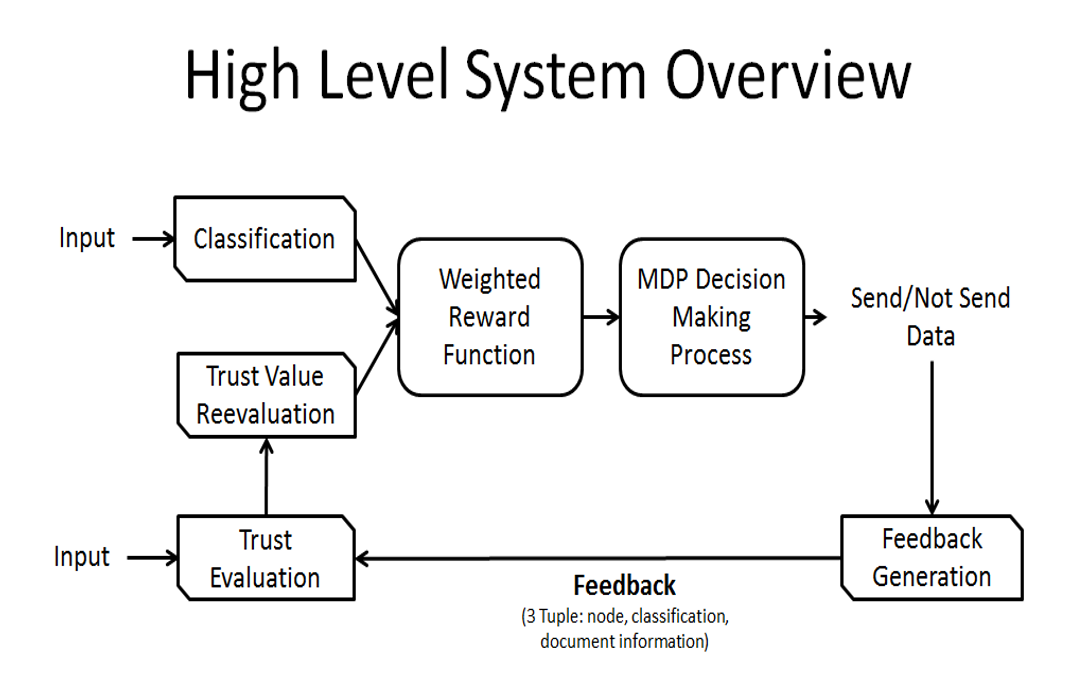
\includegraphics[width=0.90\textwidth]{Figures/HighLevelOverview.PNG}
        \caption{System Overview}
        \label{fig:SystemOverview}
    \end{center}
\end{figure}

\begin{enumerate}
    \item Classification of Data is done on a data set.
        \begin{enumerate}
            \item The input will be the data to be classified
            \item The output will be some bounded, integral value representing a classification level
        \end{enumerate}
    \item The output of this classification is used as an input of a planning function for a specific node.
    \item This Trust Evaluation function uses the similarity metric,
        classification of the document and original trust value of the node we
        are evaluating.
    \item The Trust Evaluation output is used as an input to a MDP (Markov Decision Process). 
        \begin{enumerate}
            \item This value is a real number between 0 and 1. With minumum 3 decimal points of precision.
        \end{enumerate}
    \item This MDP is able to make a binary decision on whether or not to
        recommend the transmission of certain data, between two nodes.
    Furthermore, the system is suggestive, this decision will inform the user
(node level).  
    \item If a transmission occurs between two nodes, there is feedback in the
        form of a difference function able to provide input to the Trust
    Evaluation function, who in turn makes a decision about modifying node trust values.
    The feedback of the difference function will inform the \gls{sa} to make updates on node
    trust before any new trust evaluation takes place.  
    
    \end{enumerate}

\FloatBarrier
\section{Task Breakdowns}

\begin{table}[h!]
    \centering
    \begin{tabular}{c | c }
        \hline
        Component	& Person \\
        \hline \hline
        Decision Planning Survey      & Arun Buduru \& David Lucero\\
        MDP Implementation in Matlab  & Arun Buduru  \\
                        \hline
        Data Set Research    &   Sachit Dhal\\
        Algorithm Survey     &   Jeremy Wright \\
        Classification Implementation &  Jeremy Wright \\
                        \hline
        Trust Management Equation Design &   Ashwin Nedunoori \& Abdulaziz Alnori\\
        Equation Testing &   Ashwin Nedunoori \& Abdulaziz Alnori\\
                        \hline
        Typesetting  & Jeremy Wright\\
        \hline
        Commercial Offerings Survey  & David Lucero
    \end{tabular}
    \caption{Group Member Responsibilities}
\end{table}
